\documentclass{article}
 
%encoding
%--------------------------------------
\usepackage[T1]{fontenc}
\usepackage[utf8]{inputenc}
%--------------------------------------
 
%Portuguese-specific commands
%--------------------------------------
\usepackage[portuguese]{babel}
%--------------------------------------

\usepackage{graphicx}
\usepackage{indentfirst}
\usepackage{hyperref}

\graphicspath{{img/}}

\title{Manual do Usuário D+}

\author{Lucas Ferreira de Almeida}

\date{13/10/2021}

\begin{document}

\maketitle

\tableofcontents

\pagebreak

\section{Tokens}

\subsection{Identificadores}
\begin{tabular}{ l | c }
   Identificador & ID  \\
\end{tabular}

\subsection{Literais}

\begin{tabular}{ l | c }
 Inteiros & \texttt{LIT\_INT}  \\
 Reais & \texttt{LIT\_FLT}   \\
 Caractere & \texttt{LIT\_CHAR}  \\
 String & \texttt{LIT\_STR}   \\
 Boolean & \texttt{LIT\_BOOL}  \\
\end{tabular}

\subsection{Palavras Reservadas}

\begin{tabular}{ l | c }
void & \texttt{PR\_VOID}  \\
int & \texttt{PR\_INT}  \\
float & \texttt{PR\_FLT}  \\
char & \texttt{PR\_CHAR}  \\
bool & \texttt{PR\_BOOL}  \\
if & \texttt{PR\_IF}  \\
then & \texttt{PR\_THEN}  \\
else & \texttt{PR\_ELSE}  \\
end-if & \texttt{PR\_ENDIF}  \\
for & \texttt{PR\_FOR}  \\
while & \texttt{PR\_WHILE}  \\
do & \texttt{PR\_DO}  \\
return & \texttt{PR\_RETURN}  \\
true & \texttt{PR\_TRUE}  \\
false & \texttt{PR\_FALSE}  \\
var & \texttt{PR\_VAR}  \\
main & \texttt{PR\_MAIN}  \\
scan & \texttt{PR\_SCAN}  \\
print & \texttt{PR\_PRINT}  \\
\end{tabular}

\subsection{Pontuação}

\begin{tabular}{ l | c }
, & \texttt{VIRGULA} \\
; & \texttt{PONTO\_VIRGULA} \\
( & \texttt{ABRE\_PARENTESES} \\
) & \texttt{FECHA\_PARENTESES} \\
 \texttt{[} & \texttt{ABRE\_COLCHETES} \\
 \texttt{]} & \texttt{FECHA\_COLCHETES} \\
 \texttt{\{} & \texttt{ABRE\_CHAVES} \\
 \texttt{\}} & \texttt{FECHA\_CHAVES} \\
\end{tabular}

\subsection{Operadores}

\begin{tabular}{ l | c }
 + & \texttt{OP\_SOMA} \\
 - & \texttt{OP\_SUB} \\
 \texttt{*} & \texttt{OP\_MULT} \\
 / & \texttt{OP\_DIV} \\
 \% & \texttt{OP\_MOD} \\
 ? & \texttt{OP\_TER} \\
 ! & \texttt{OP\_NEG} \\
 . & \texttt{OP\_PONTO} \\
 < & \texttt{OP\_MENOR} \\
 > & \texttt{OP\_MAIOR} \\
 == & \texttt{OP\_IGUAL} \\
 != & \texttt{OP\_DIF} \\
 <= & \texttt{OP\_MEN\_IGUAL} \\
 >= & \texttt{OP\_MAI\_IGUAL} \\
 = & \texttt{OP\_ATRI} \\
 += &  \texttt{OP\_ADIC\_IGUAL} \\
 -= &  \texttt{OP\_SUB\_IGUAL} \\
 ++ &  \texttt{OP\_INC} \\
 - - &  \texttt{OP\_DEC} \\
\&\& &  \texttt{OP\_AND} \\
 || &  \texttt{OP\_OR} \\
\end{tabular}

\pagebreak

\section{Diagramas de transição}

\subsection{Identificadores}

\begin{figure}[!h]
\centering
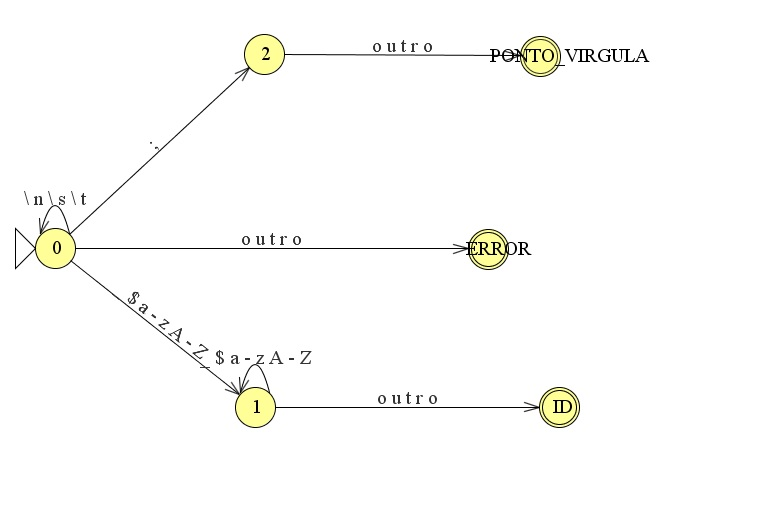
\includegraphics[width=10cm]{DT_ID.jpg}
\caption{Indetificadores.}
\label{fig:CL_logo}\end{figure}

\subsection{Literais}

\begin{figure}[!h]
\centering
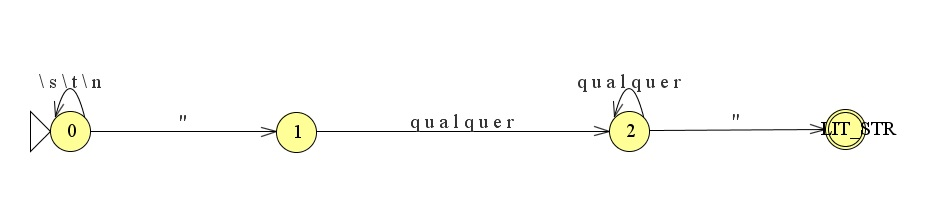
\includegraphics[width=12cm]{DT_LIT_STR.jpg}
\caption{Literais (String).}
\label{fig:CL_logo}\end{figure}

\pagebreak

\begin{figure}[!h]
\centering
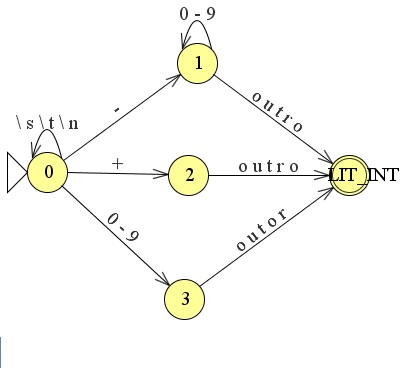
\includegraphics[width=9cm]{DT_LIT_INT.jpg}
\caption{Literais (Inteiro).}
\label{fig:CL_logo}\end{figure}

\begin{figure}[!h]
\centering
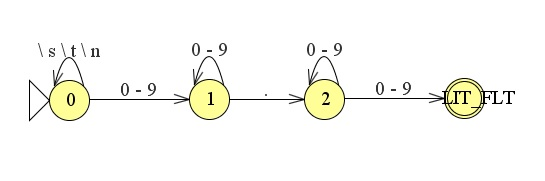
\includegraphics[width=10cm]{DT_LIT_FLT.jpg}
\caption{Literais (Reais).}
\label{fig:CL_logo}\end{figure}

\pagebreak

\begin{figure}[!h]
\centering
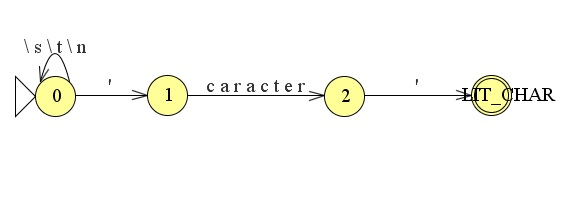
\includegraphics[width=9cm]{DT_LIT_CHAR.jpg}
\caption{Literais (Char).}
\label{fig:CL_logo}\end{figure}

\begin{figure}[!h]
\centering
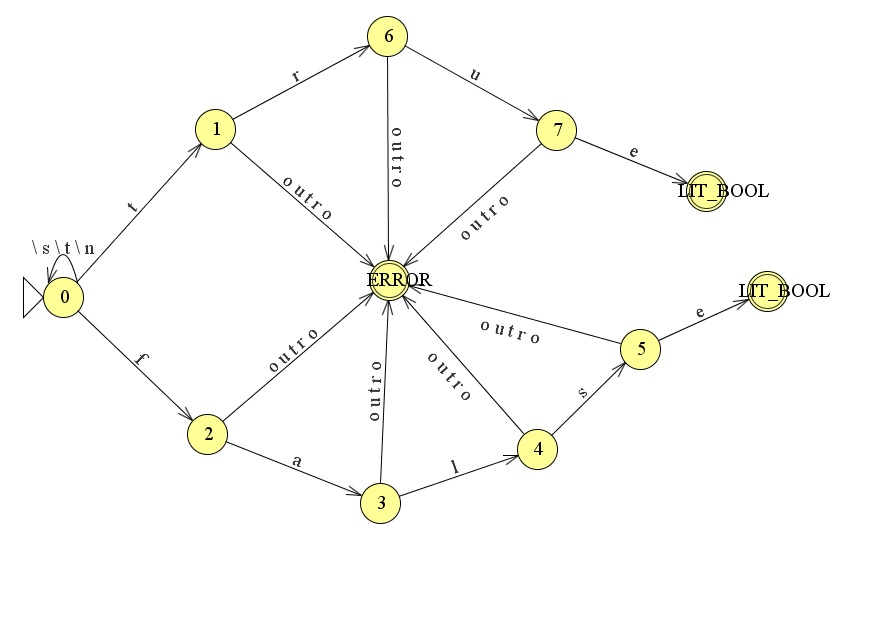
\includegraphics[width=12cm]{DT_LIT_BOOL.jpg}
\caption{Literais (Boolean).}
\label{fig:CL_logo}\end{figure}

\pagebreak

\subsection{Pontuação}

\begin{figure}[!h]
\centering
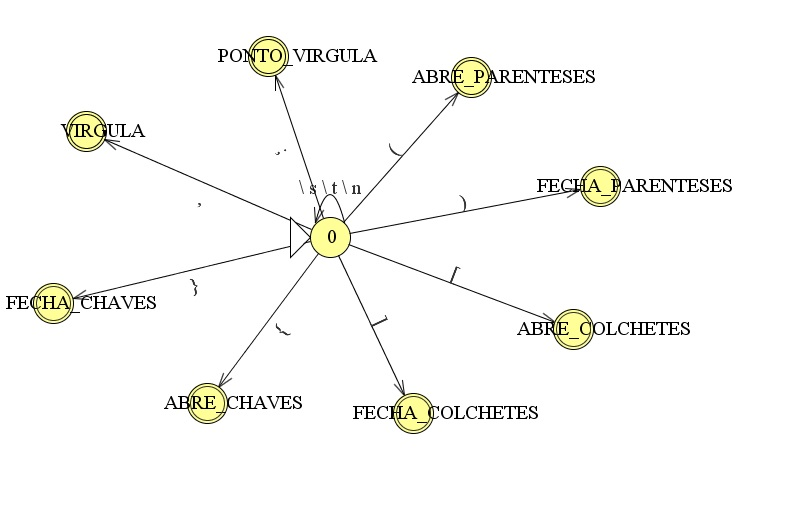
\includegraphics[width=12cm]{DT_Pontuacao.jpg}
\caption{Literais (Boolean).}
\label{fig:CL_logo}\end{figure}

\subsection{Palavras Reservadas}

\begin{figure}[!h]
\centering
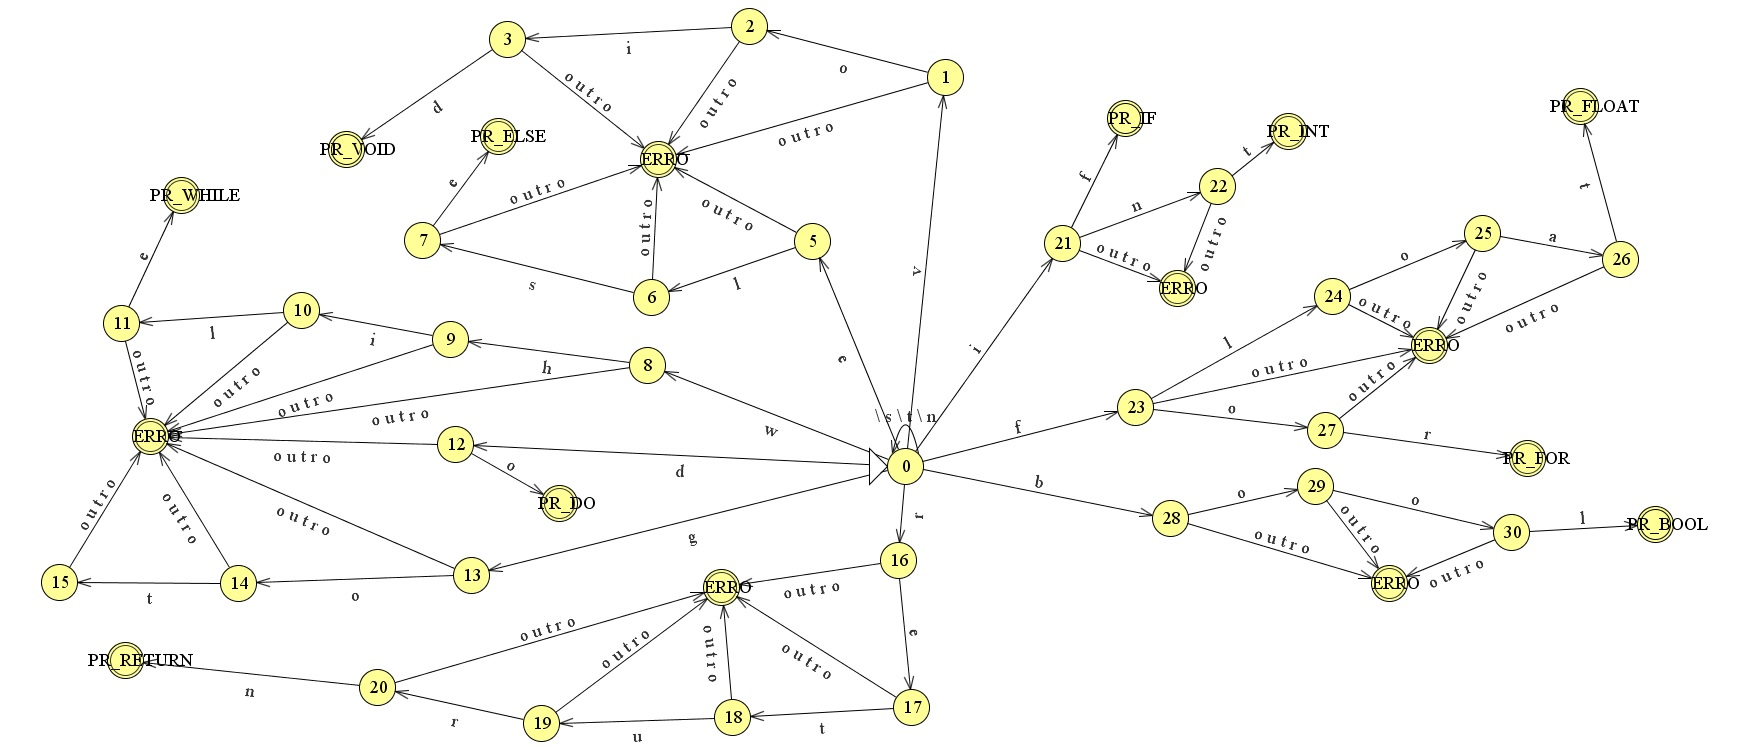
\includegraphics[width=15cm]{DT_PALAVRAS_RESERV.jpg}
\caption{Literais (Boolean).}
\label{fig:CL_logo}\end{figure}

\pagebreak

\subsection{Operadores}

\begin{figure}[!h]
\centering
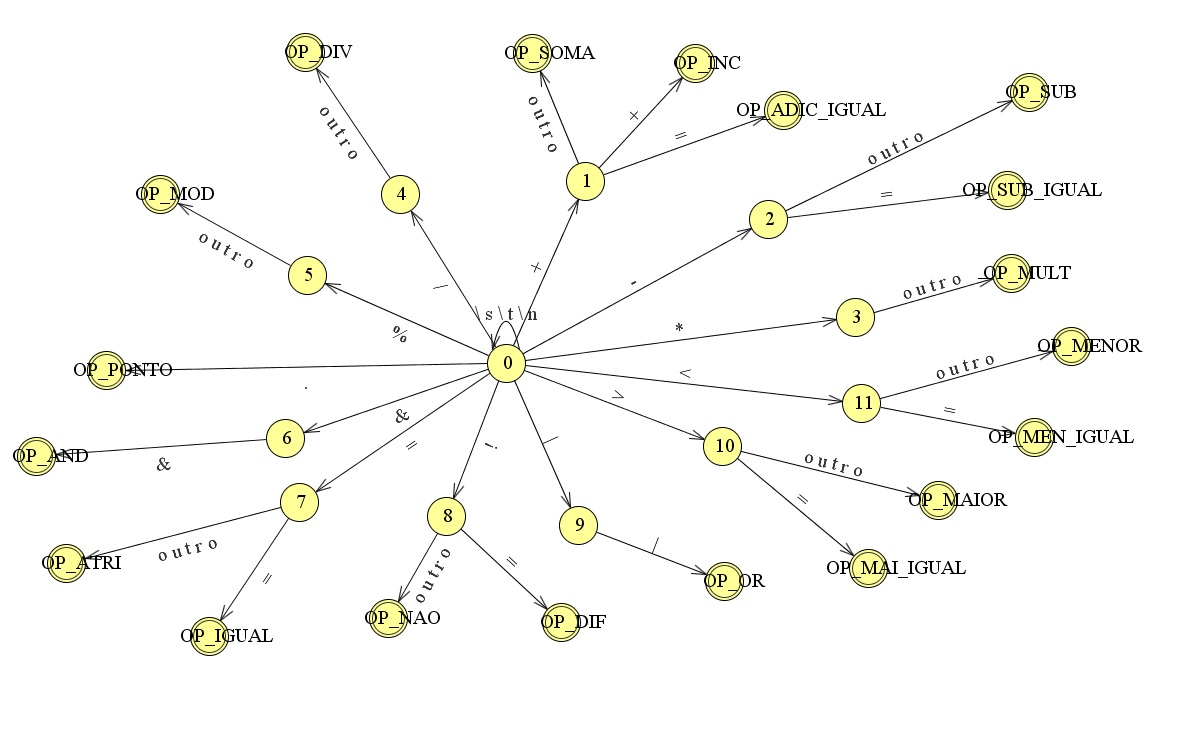
\includegraphics[width=15cm]{DT_OPERADORES.jpg}
\caption{Literais (Boolean).}
\label{fig:CL_logo}\end{figure}

\end{document}